\appendix
% %%%%%%%%%%%%%%%%%%%%%%%%%%%%%%%%%%%%%%%%%%%%%%%%%%%%%%%%%%%%%%%%%%%%%%
% First appendix
% %%%%%%%%%%%%%%%%%%%%%%%%%%%%%%%%%%%%%%%%%%%%%%%%%%%%%%%%%%%%%%%%%%%%%%
\fancychapter{Appendix A}
\label{ch:rsom_training}
\begin{figure}[htpb]
  \centering
  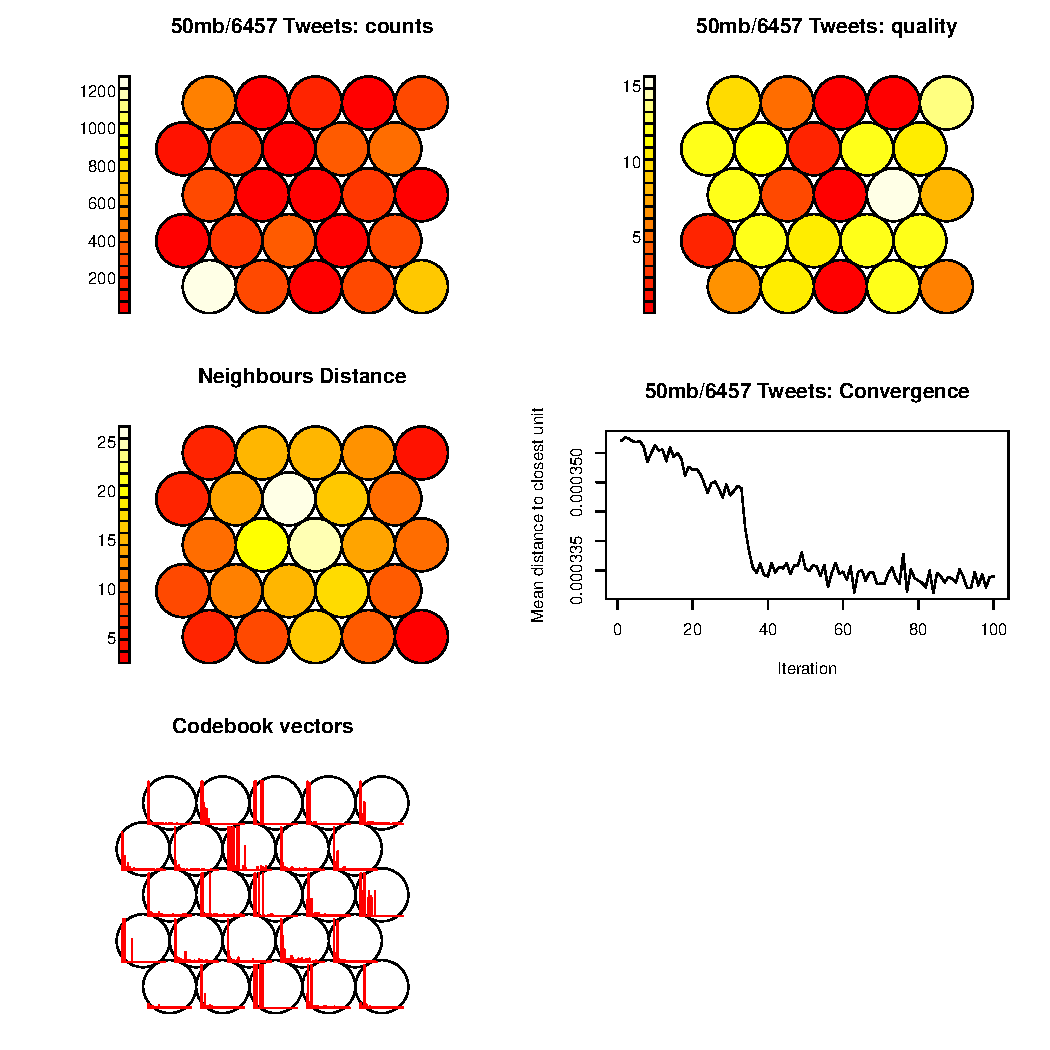
\includegraphics[width=0.8\linewidth]{./images/50mb_6457tweets_dataset.pdf}
  \caption{Training data for 6457 tweets. The counts map, shows us how many tweets are mapped to each cluster. Quality shows the mean distance of objects mapped to a unit to the codebook vector, the smaller the distance the better the representation. The neighborhood disance show the U-Matrix and finally the tweets convergence shows the distance from each node's wheights to the samples represented by that node }
  \label{fig:somr_images}
\end{figure}

\cleardoublepage

% %%%%%%%%%%%%%%%%%%%%%%%%%%%%%%%%%%%%%%%%%%%%%%%%%%%%%%%%%%%%%%%%%%%%%%
% Second appendix
% %%%%%%%%%%%%%%%%%%%%%%%%%%%%%%%%%%%%%%%%%%%%%%%%%%%%%%%%%%%%%%%%%%%%%%
%\fancychapter{Appendix A}
%\cleardoublepage  
